\documentclass[12pt]{article}

\usepackage{sbc-template}
\usepackage{graphicx,url}
\usepackage{amsmath}
\usepackage[utf8]{inputenc}
\usepackage[brazil]{babel}

     
\sloppy

\title{Análise Visual Interativa da Acessibilidade no Cenario Cinematográfico Brasileiro}

\author{ Amanda Júlia Ferreira\inst{1}, Ana Vitória Vaz Santos\inst{1}, Lucas Gabriel Alves Ferreira\inst{1} }


\address{Faculdade de Computação -- Universidade Federal do Uberlândia (UFU) \\ Uberlândia -- MG -- Brazil
  \email{\{amanda.julia,vitoria.vaz,lucas.ferreira3\}@ufu.br}
}

\begin{document} 

\maketitle
     
\begin{resumo} 
  Este trabalho apresenta um sistema web interativo para exploração e análise 
  de dados de acessibilidade nas salas de cinema do Brasil, utilizando dados 
  abertos da Agência Nacional do Cinema (ANCINE). A partir da arquitetura do 
  pipeline clássico de visualização de dados, foi desenvolvido um ecossistema 
  com três layouts coordenados e implementados exclusivamente com a biblioteca 
  D3.js: um mapa coroplético enriquecido com glifos temáticos, um gráfico de 
  dispersão com painel estatístico e brushing bidimensional, e um diagrama de 
  funil trapezoidal para retenção de conformidade. A ferramenta permite 
  identificar disparidades regionais de infraestrutura e capacidade de atendimento, 
  auxiliando a tomada de decisão para políticas públicas e investimentos privados.
\end{resumo}


\section{Introdução}

O acesso à cultura e ao lazer é um direito fundamental estipulado por diretrizes 
nacionais e internacionais de inclusão social. No contexto do entretenimento audiovisual, 
garantir que complexos cinematográficos ofereçam acessibilidade física e espacial 
apropriada é indispensável para promover a autonomia de pessoas com deficiência, 
mobilidade reduzida ou obesidade. 

A Agência Nacional do Cinema (ANCINE) disponibiliza 
dados abertos detalhados sobre o parque exibidor brasileiro. Contudo, tabelas puramente 
numéricas dificultam a identificação de padrões espaciais, assimetrias regionais e gargalos 
na jornada do espectador.

Neste trabalho, propõe-se um sistema de análise visual interativo web, 
fundado no processo clássico de visualização de dados, que transforma dados brutos da ANCINE 
em representações gráficas enriquecidas. A solução adota metáforas visuais avançadas e 
ferramentas de interação inter-relacionadas (como brushing \& linking e filtragem geográfica), 
desenvolvidas estritamente com a biblioteca D3.js. 

\section{Objetivos}

\subsection{Objetivo Geral}

Desenvolver e aplicar um sistema de análise visual interativo baseado em web para mapear, 
comparar e explorar a acessibilidade física e a capacidade de assentos adaptados em salas 
de cinema de todas as Unidades Federativas (UFs) do Brasil.

\subsection{Objetivos Específicos}
\begin{itemize}
    \item Pré-processar e estruturar a base de dados da ANCINE, calculando métricas compostas de infraestrutura e capacidade de atendimento;
    \item Implementar três layouts gráficos avançados no D3.js que superem a limitação de gráficos básicos de barras ou setores:
    \begin{itemize}
        \item Mapa Choropleth-Glyph para análise espacial e multiatribuição geográfica;  
        \item Scatter Plot Interativo com Painel KPI para exploração de relações entre capacidade e proporção de assentos reservados;
        \item Funil de Conformidade Sequencial para avaliar os gargalos da jornada de acessibilidade física;
    \end{itemize}
    \item Prover mecanismos de interação rica (hovering, tooltips informativos, filtragem por clique e seleção por área com brushing bidimensional);
    \item Extrair insights relevantes sobre as disparidades regionais de acessibilidade no território brasileiro.
\end{itemize}

\section{Pipeline de Visualização e Pré-Processamento dos Dados}

A construção da ferramenta seguiu rigorosamente o modelo de Pipeline de Visualização:

\[
\text{Dados Brutos} \longrightarrow \text{Tabelas de Dados} \longrightarrow \text{Estruturas Visuais} \longrightarrow \text{Visões \& Interação}
\]

\subsection{Tratamento e Engenharia de Atributos em Python}

A base bruta continha registros detalhados por sala de exibição. 
Um script em Python (pre_processar_ancine.py) executou as seguintes transformações:

\begin{enumerate}
    \item Cálculo de Proporções Relativas: Para evitar viés de escala em salas grandes vs. pequenas, foram computadas as taxas de assentos acessíveis:
    \subitem $$\text{prop\_cad} = \frac{\text{Assentos Cadeirantes}}{\text{Assentos Totais}}$$
    \subitem $$\text{prop\_mob} = \frac{\text{Assentos Mobilidade Reduzida}}{\text{Assentos Totais}}$$
    \subitem $$\text{prop\_obe} = \frac{\text{Assentos Obesidade}}{\text{Assentos Totais}}$$ 
    \item Tratamento de Outliers e Normalização Global: Para combater distorções de valores extremos no reescalonamento Min-Max, aplicou-se um corte (clipping) no percentil 99 ($p_{99}$) das proporções antes da normalização para a escala $[0, 1]$:
    \subitem $$\text{norm\_col} = \frac{\text{clip}(x, 0, p_{99}) - \min}{\max - \min}$$
    \item Geração de Scores Compostos:
      \begin{itemize}
          \item Score de Infraestrutura ($\text{score\_infra}$): Média aritmética simples de três variáveis binárias ($0$ ou $1$): presença de rampa de acesso à sala, rampa de acesso aos assentos e banheiros acessíveis.
          \item Score de Capacidade ($\text{score\_capacidade}$): Média das proporções normalizadas dos três tipos de assentos adaptados.
      \end{itemize}
    \item Exportação Hierárquica em JSON: Os dados foram estruturados em 5 JSONs leves otimizados para rápida renderização no lado do cliente (client-side) com D3.js: agregações por UF, Exibidor, Complexo, Funil e Nível de Sala.
\end{enumerate}

\section{Detalhamento da Proposta e Metáforas Visuais}

A interface é composta por três visões integradas. O design visual apoiou-se em Princípios de Gestalt 
e Atributos Pré-atentivos (cor, tamanho e posição) para otimizar a carga cognitiva.

\subsection{Layout 1: Mapa Choropleth-Glyph (Análise Espacial Bivariada)}

\begin{itemize}
    \item Metáfora Visual: Representação cartográfica do território brasileiro em que cada UF atua como 
    um contêiner geográfico.
    \item Mapeamento de Canais Visuais:
          \begin{itemize}
              \item Matiz/Saturação (Área do Estado): Gradiente linear de azul (d3.scaleLinear) representando 
              o $\text{score\_infra\_medio}$. Tons mais escuros direcionam a atenção pré-atentiva para estados 
              com melhor infraestrutura. 
              \item Glifo Temático (Câmera de Cinema): Posicionado no centroide geométrico de cada UF (d3.geoPath().centroid).
              \item Tamanho do Glifo: Codificado via escala de raiz quadrada (d3.scaleSqrt) pela quantidade de salas na UF (qtd_salas), 
              garantindo proporcionalidade de área perceptiva e evitando a distorção do crescimento de raio.
              \item Cor do Glifo: Escala sequencial de laranjas (d3.interpolateOranges) refletindo o $\text{score\_capacidade\_medio}$.
          \end{itemize}
    \item Fundamentação de Percepção (Gestalt):
          \begin{itemize}
              \item Segregação Figura-Fundo: O traço contínuo dos estados e o contorno branco dos glifos garantem legibilidade sobre o fundo.
              \item Proximidade: A centralização do glifo no centroide vincula visualmente o ícone ao seu respectivo estado.
          \end{itemize}
\end{itemize}

\subsection{Layout 2: Distribuição de Salas com Brushing e KPIs (Análise Multivariada)}

\begin{itemize}
    \item Metáfora Visual: Plano cartesiano de dispersão (Scatter Plot) acompanhado por um dashboard de indicadores estatísticos.
    \item Mapeamento de Canais Visuais:
    \begin{itemize}
      \item Eixo X (Posição Horizontal): Quantidade total de assentos por sala ($0$ a $1800$).  
      \item Eixo Y (Posição Vertical): Percentual de assentos destinados a cadeirantes ($0\%$ a $40\%$). 
      \item Cor do Ponto: Intensidade de azul proporcional ao $\text{score\_infra}$ individual da sala. 
    \end{itemize}
    \item Painel Estatístico Vinculado: Exibe KPIs como a taxa de "Jornada Acessível Completa" 
    (presença simultânea de rampa de acesso, rampa aos assentos e banheiro acessível) e a contagem total de assentos adaptados.
\end{itemize}

\subsection{Layout 3: Funil Sequencial de Conformidade (Análise Processual)}

\begin{itemize}
    \item Metáfora Visual: Funil contínuo composto por polígonos trapezoidais (<polygon> no SVG), 
    simbolizando a filtragem e retenção ao longo das etapas da experiência física do espectador.
    \item Mapeamento de Canais Visuais:
    \begin{itemize}
    \item Largura das Bases: Mapeada linearmente (d3.scaleLinear) pelo volume de salas que atendem aos critérios.
    \item Gradação de Cor: Escala d3.interpolateBlues que se intensifica conforme as exigências aumentam.
    \end{itemize}
    \item Significado das Etapas:
    \begin{enumerate}
    \item Base Total: 100% das salas catalogadas.
    \item Acesso à Sala com Rampa: Salas que possuem rampa de entrada.
    \item Assentos com Rampa: Salas que possuem rampa interna até as poltronas.
    \item Sanitários Acessíveis: Salas integradas a complexos com banheiros adaptados (Acessibilidade Plena).
    \end{enumerate}

\end{itemize}

The subsection titles must be in boldface, 12pt, flush left.

\section{Figures and Captions}\label{sec:figs}


Figure and table captions should be centered if less than one line
(Figure~\ref{fig:exampleFig1}), otherwise justified and indented by 0.8cm on
both margins, as shown in Figure~\ref{fig:exampleFig2}. The caption font must
be Helvetica, 10 point, boldface, with 6 points of space before and after each
caption.

\begin{figure}[ht]
\centering
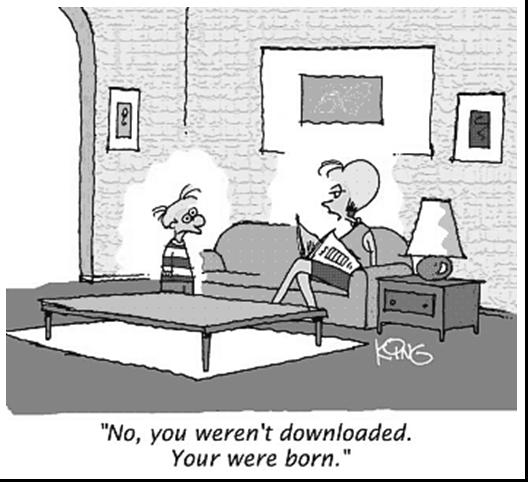
\includegraphics[width=.5\textwidth]{fig1.jpg}
\caption{A typical figure}
\label{fig:exampleFig1}
\end{figure}

\begin{figure}[ht]
\centering
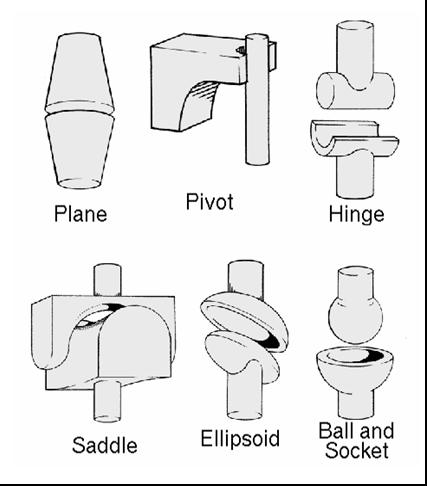
\includegraphics[width=.3\textwidth]{fig2.jpg}
\caption{This figure is an example of a figure caption taking more than one
  line and justified considering margins mentioned in Section~\ref{sec:figs}.}
\label{fig:exampleFig2}
\end{figure}

In tables, try to avoid the use of colored or shaded backgrounds, and avoid
thick, doubled, or unnecessary framing lines. When reporting empirical data,
do not use more decimal digits than warranted by their precision and
reproducibility. Table caption must be placed before the table (see Table 1)
and the font used must also be Helvetica, 10 point, boldface, with 6 points of
space before and after each caption.

\begin{table}[ht]
\centering
\caption{Variables to be considered on the evaluation of interaction
  techniques}
\label{tab:exTable1}
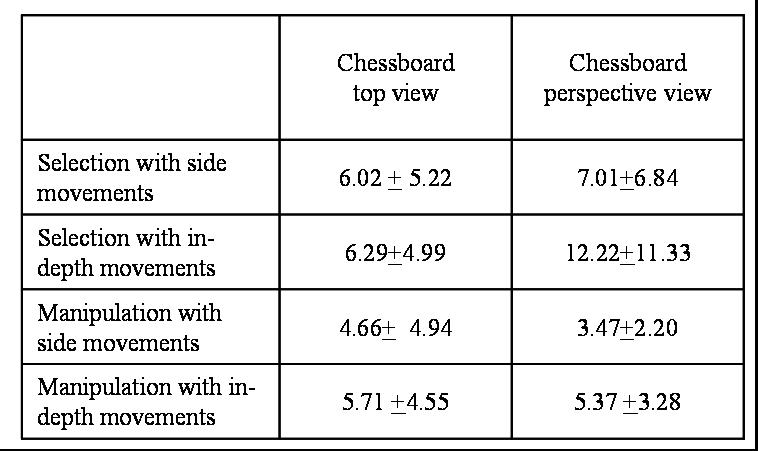
\includegraphics[width=.7\textwidth]{table.jpg}
\end{table}

\section{Images}

All images and illustrations should be in black-and-white, or gray tones,
excepting for the papers that will be electronically available (on CD-ROMs,
internet, etc.). The image resolution on paper should be about 600 dpi for
black-and-white images, and 150-300 dpi for grayscale images.  Do not include
images with excessive resolution, as they may take hours to print, without any
visible difference in the result. 

\section{References}

Bibliographic references must be unambiguous and uniform.  We recommend giving
the author names references in brackets, e.g. \cite{knuth:84},
\cite{boulic:91}, and \cite{smith:99}.

The references must be listed using 12 point font size, with 6 points of space
before each reference. The first line of each reference should not be
indented, while the subsequent should be indented by 0.5 cm.

\bibliographystyle{sbc}
\bibliography{sbc-template}

\end{document}
